\appendix

\section[]{Backup}

\begin{frame}[plain]
\begin{center}
\textbf{\Large Backup}
\end{center}
\end{frame}

\begin{frame}[plain]
\frametitle{Remains to be done}
\begin{maliste}
\item Add backup (or put it in the corps du texte ?) on same-sign dilepton excess (arXiv:1507.0160 may be a good starting point)
\item Slides diff analyse partielle / analyse complete (cf debut chap 8 these 
Loic)
\item Add slide with run 2 prospects (increase in xsec for signals and backgrounds, preliminary sensitivities, lumi to achieve run 1 results, ...)
\item Limites en metres
\item re-read my theoretical summary
\item likelihood fakes
\end{maliste}

\end{frame}

\begin{frame}
\frametitle{JER 2012}
\begin{center}
\includegraphics[width=0.5\textwidth]{Figures/JES/JERplot2012.png}
\includegraphics[width=0.5\textwidth]{Figures/JES/JERvalues2012.png}
\end{center}
\end{frame}

\begin{frame}[plain]
\frametitle{EM+JES uncertainty}
\begin{center}
\includegraphics[width=0.7\textwidth]{Figures/JES/fig_22a_JES2010UncertaintyCentral.pdf}
\end{center}
\end{frame}

\begin{frame}[plain]
\frametitle{Phénoménologie 2UED/RPP}
\begin{maliste}
\item Désintégration : 
\begin{itemize}
\item $(1,0)\rightarrow A^{(0,1)} + SM$
\vspace*{0.2cm}
\item $(1,1)\rightarrow (1,1) + SM$\\
$(1,1)\rightarrow SM + SM$ (opérateur ordre supérieur)\\
$(1,1)\rightarrow (1,0)+(0,1)$ interdit (sous seuil cinématique)
\vspace*{0.2cm}
\item $(2,0)\rightarrow (2,0) + SM$\\
$(2,0)\rightarrow SM + SM$ \\
$(2,0)\rightarrow (1,0) + (1,0)$
\end{itemize}
\vspace*{0.2cm}
\item Production (dominée par QCD $\rightarrow$ quarks et gluons dans état final)
\begin{itemize}
\item $pp\rightarrow (1,0)+(1,0)$
\item $pp\rightarrow (1,1)+(1,1)$
\item $pp\rightarrow (2,0)+(2,0)$
\end{itemize}
\end{maliste}
\end{frame}

\begin{frame}[plain]
\frametitle{Phénoménologie 2UED/RPP}
\[m_{(n,0)/(0,n)}^2=\frac{1}{R_{4/5}^2}\left(n^2+m_{SM}^2R_{4/5}^2+\delta_\text{finite}^{(n,0)/(0,n)}\left(R_4,R_5\right)+n^2\delta_{log}\right)\]
avec 
\[\delta_{log}\sim \log\Lambda R_{4/5}\]

\[m_{H^{(2,0)/(0,2)}}^2=\frac{1}{R_{4/5}^2}\left(n^2+m_{SM}^2R_{4/5}^2+m_{loc}^2R_{4/5}^2+\delta_\text{finite}^{(2,0)/(0,2)}\left(R_4,R_5\right)+4\delta_{log}\right)\]
\end{frame}

\begin{frame}[plain]
\frametitle{Phénoménologie 2UED/RPP}
\begin{maliste}
\item Contraintes issues de réinterprétation d'analyse run 1 d'ATLAS et CMS :
\begin{itemize}
\item tier : $(1,0)$, MET searches (single lepton, same-sign, opposite-sign), arXiv:1302.4750 : $m_{KK}\gtrsim 600~$GeV  
\item tier : $(2,0)$, arXiv:1209.6556
\begin{center}
\includegraphics[width=0.5\textwidth]{Figures/FourTops/reinterpretation2UEDRPPtier20.png}\\
\includegraphics[width=0.7\textwidth]{Figures/FourTops/reinterpretation2UEDRPPtier20_resultats.png}
\end{center}
\end{itemize}
\end{maliste}
\end{frame}

\begin{frame}[plain]
\frametitle{Phénoménologie 2UED/RPP : matière noire}
\begin{maliste}
\item Dark matter candidate :
\begin{itemize}
\item Lighest particule for $m_{KK}>200$~GeV : $A^{(1,0)}$, $A^{(0,1)}$
\item Lighest particule for $m_{KK}<200$~GeV : $e_S^{(1,0)}$, $e_S^{(0,1)}$
\end{itemize}
\vspace*{0.2cm}
Remark : for chiral square or mUED, lightest particle is $h^{(1,0)}$ (this mode vanishes on the RPP, so we don't need to consider it as a DM candidate).\\
\vspace*{0.5cm}
\item Lightest particles of tier $(2,0)$ : $A^{(2,0)}$ and $H^{(2,0)}$ \\
These particles do not decay into any KK excitations\\
$\rightarrow$ This strongly reduces relic abundance
\vspace*{0.5cm}
\item Decoupling limit : $R_4 \gg R_5$\\
$\rightarrow$ all particles from tier $(0,n)$ decouple from theory (very large mass) and don't interact with ordinary matter or particles from tier $(n,0)$\\
$\rightarrow$ DM candidate is $A^{(1,0)}$ (interacts with all particles from tier $(n,0)$ and SM)
\item Symmetric case : $R_4 = R_5$\\
$\rightarrow$ Two DM candidates not interacting with each other : $A^{(1,0)}$ and $A^{(0,1)}$
\end{maliste}
\end{frame}

\begin{frame}[plain]
\frametitle{Phénoménologie 2UED/RPP : abondance relique - détection directe}
\begin{maliste}
\item Processus d'annihilation :
\begin{itemize}
\item $A^{(1,0)}+A^{(1,0)}\rightarrow ZZ$ 
\item $A^{(1,0)}+A^{(1,0)}\rightarrow W^+W^-$ 
\item $A^{(1,0)}+A^{(1,0)}\rightarrow HH$ 
\item $A^{(1,0)}+A^{(1,0)}\rightarrow $fermions 
\end{itemize}
\vspace*{0.2cm}
\item Evolution abondance relique avec $\Lambda R$ (pour $m_{KK}$ donné) :\\
$\rightarrow$ varier $\Lambda$ fait varier les masses et donc section eff. (co)-annihilation\\
$\rightarrow$ on a : section eff. (co)-annihilation augmente lorsque $\Lambda$ augmente\\
$\Rightarrow$ abondance relique décroît avec $\Lambda$
\vspace*{0.2cm}
\item Evolution sensibilité détection directe avec $\Lambda R$ (pour $m_{KK}$ donné) :\\
$\rightarrow$ section eff. $A^{(1,0)}+\text{SM}$ décroît avec $\Lambda$
$\Rightarrow$ sensibilité détection directe décroît avec $\Lambda$
\end{maliste}
\end{frame}



\begin{frame}[plain]
\frametitle{MS dans bulk}
Slide taken from Charles Bouchart et Gregory Moreau
\begin{figure}[!htb]
\begin{center}
\hspace*{-1cm}
\includegraphics[width=1.05\textwidth]{Figures/FourTops/SMdansBulkProfiles.png}
\end{center}
\end{figure}
\end{frame}

\begin{frame}[plain]
\frametitle{2HDM four tops production}
\begin{maliste}
\item P. S. Bhupal, Maximally Symmetric 2HDM model with natural standard model alignment, arXiv:1408.3405
\item 2HDM : 5 degrees of freedom (2 CP-even scalars ($H,h$), CP-odd pseudoscalar ($A$), 2 charged Higgs $H^\pm$)
\item Type II (MSSM-like) : u-type and d-type couple to different doublets
\item Heavy CP-even higgs gaugephobic in MS-2HDM
\begin{itemize}
\item Couples mainly to fermions
\item Produces mainly by ggF and associate production with $t\bar{t}$ ($b\bar{b}$) at low (high) $\tan\beta$ (VBF and associate productions suppressed)
\item[$\rightarrow$] $h\rightarrow t\bar{t}$ main decay mode over most of parameter space for $\tan\beta\leq5$
\end{itemize}
\end{maliste}
\end{frame}

\begin{frame}[plain]
\frametitle{2HDM four tops production}

arXiv:1408.3405
\begin{figure}[!htb]
\begin{center}
\hspace*{-1cm}
\includegraphics[width=1.1\textwidth]{Figures/FourTops/2HDM_TypeII_4tops_XsecVsMh.png}
\end{center}
\end{figure}

\end{frame}

\begin{frame}[plain]
\frametitle{Event selection : preselection}
\begin{small}
\begin{maliste}
\item Common criteria :
\begin{itemize}
\item Single lepton trigger (EF\_e24vhi\_medium1, EF\_e60\_medium1, EF\_mu24i\_tight or EF\_mu36\_tight)
\item $\geq$ 1 primary vertex ($\geq 5$ tracks with $p_T>0.4~$GeV, highest $\sum p_T^2$)
\item Quality criteria (GRL, no overlap between $e$ and $\mu$, no bad jet, no LAr noise burst, no cosmics, ...)
\item $\geq$ 1 jet ($p_T>25$~GeV, $|\eta|<2.5$)
\end{itemize}
\item Same-sign dilepton channel :
\begin{itemize}
\item 2 of the 3 highest $p_T$ leptons are tight 
\item same electric charge
\item if $e^{\pm}e^{\pm}$, apply quarkonia/Z-veto : $m_{ee}>15$~GeV and $|m_{ee}-91~\text{GeV}|>10~GeV$
\item one of the two leptons matches the trigger
\end{itemize}
\item Trilepton channel :
\begin{itemize}
\item 3 highest $p_T$ leptons are tight 
\item one of the three leptons matches the trigger
\end{itemize}
\end{maliste}
\end{small}
\end{frame}

\begin{frame}
\frametitle{Estimation des \english{fakes}}
\begin{maliste}
\item \english{fakes}=leptons non-prompts
\item Source de \english{fakes} : 
\begin{itemize}
\item désintégration semi-leptonique des quarks lourds
\item conversion de photons
\item électrons tridents
\item leading $\pi^0$
\item photon associé à une trace
\end{itemize}
\item M\'ethode utilis\'ee : m\'ethode de la matrice
\vspace*{0.5cm}
\begin{center}
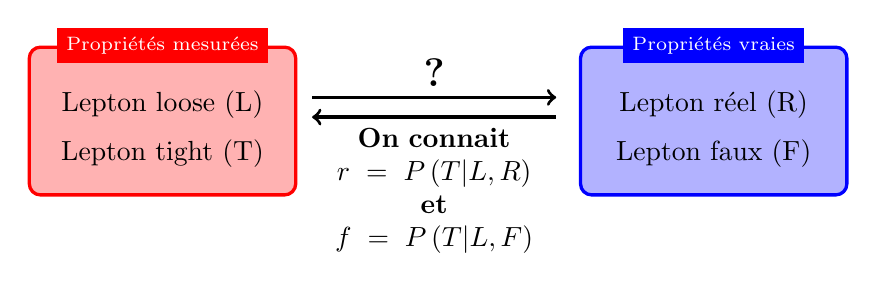
\begin{tikzpicture}
\begin{scope}
\node [draw=red, fill=red!30, very thick,
    rectangle, rounded corners, inner sep=5pt, inner ysep=10pt] (box){%
\begin{minipage}{0.25\textwidth}
\begin{center}
	\vspace*{0.2cm}	
       	Lepton loose (L) \\
       	\vspace*{0.2cm}
        Lepton tight (T)
\end{center}
\end{minipage}
};
\node[fill=red, text=white] at (box.north) {\scriptsize{Propriétés mesurées}};
\end{scope}
\draw[very thick, ->] (1.9,0.3) -- node[above, text width=4cm, align=center]
    {\Large{\bf ?}} (5,0.3);
\begin{scope}[shift={(7,0)}]
\node [draw=blue, fill=blue!30, very thick,
    rectangle, rounded corners, inner sep=5pt, inner ysep=10pt] (box){%
\begin{minipage}[t!]{0.25\textwidth}
\begin{center}
	\vspace*{0.2cm}	
       	Lepton réel (R) \\
       	\vspace*{0.2cm}
        Lepton faux (F)
\end{center}
\end{minipage}
};
\node[fill=blue, text=white] at (box.north) {\scriptsize{Propriétés vraies}};
\end{scope}
\pause
\draw[very thick, <-] (1.9,0.05) -- node[below, text width=4cm, align=center]
    {\bf On connait \\ $r = P\left(T|L,R\right)$ \\ et \\ $f=P\left(T|L,F\right)$} (5,0.05);
\end{tikzpicture}
\end{center}
%\vspace*{0.5cm}

\end{maliste}
\end{frame}

\begin{frame}
\frametitle{Estimation des \english{fakes} : définition des échantillons loose et tight}
\begin{maliste}
\item \'Echantillon tight : sélection finale de l'analyse
\item \'Echantillon loose : 
\begin{itemize}
\item Muons : loose = tight sans critères d'isolations
\item \'Electrons : loose = relachement electron ID tight++ $\rightarrow$ medium++ (en gardant le veto sur les conversions de photons)
\end{itemize}
\item Différences entre tight++ et medium++ pour électrons : $|d_0|$ (5~mm dans medium++ et 1~mm dans tight++), $\Delta\Phi(\text{track,cluster})$, $E/p$ (absent de medium++), critères d'isolation enlevés

\end{maliste}
\end{frame}

\begin{frame}
\frametitle{Estimation des \english{fakes} : détermination de $r$ et $f$}
\begin{maliste}
\item Détermination de $r$ et $f$ pour les électrons : 
\begin{itemize}
\item événements pour $r$ : 1 électron, $\ETmiss>150$~GeV
\item événements pour $f$ : 1 électron, $m_T(W)<20$~GeV, $\ETmiss+m_T(W) < 60$~GeV
\item paramétrisation : $|\eta|$, $p_T$ leading jet, $\Delta R(e,\text{nearest jet})$ (produit 1-dim)
\end{itemize}
\item Détermination de $r$ et $f$ pour les muons :
\begin{itemize}
\item événements pour $r$ : 1 muon, $m_T(W)>100$~GeV
\item événements pour $f$ : $\geq$ 2 jets, IP significance $>5$ 
\item paramétrisation : $|\eta|$, $p_T$ muon, $\Delta R(\mu,\text{nearest jet})$ (produit 1-dim)
\end{itemize}
\item Pour détermination de $f$ : contribution des leptons réels ($t\bar{t}$, single-top, $V$+jets, $VV$) soustraite par MC
\end{maliste}
\end{frame}

\begin{frame}
\frametitle{Estimation des \english{fakes} : $r$ et $f$}

\begin{figure}[!htb]
\begin{center}
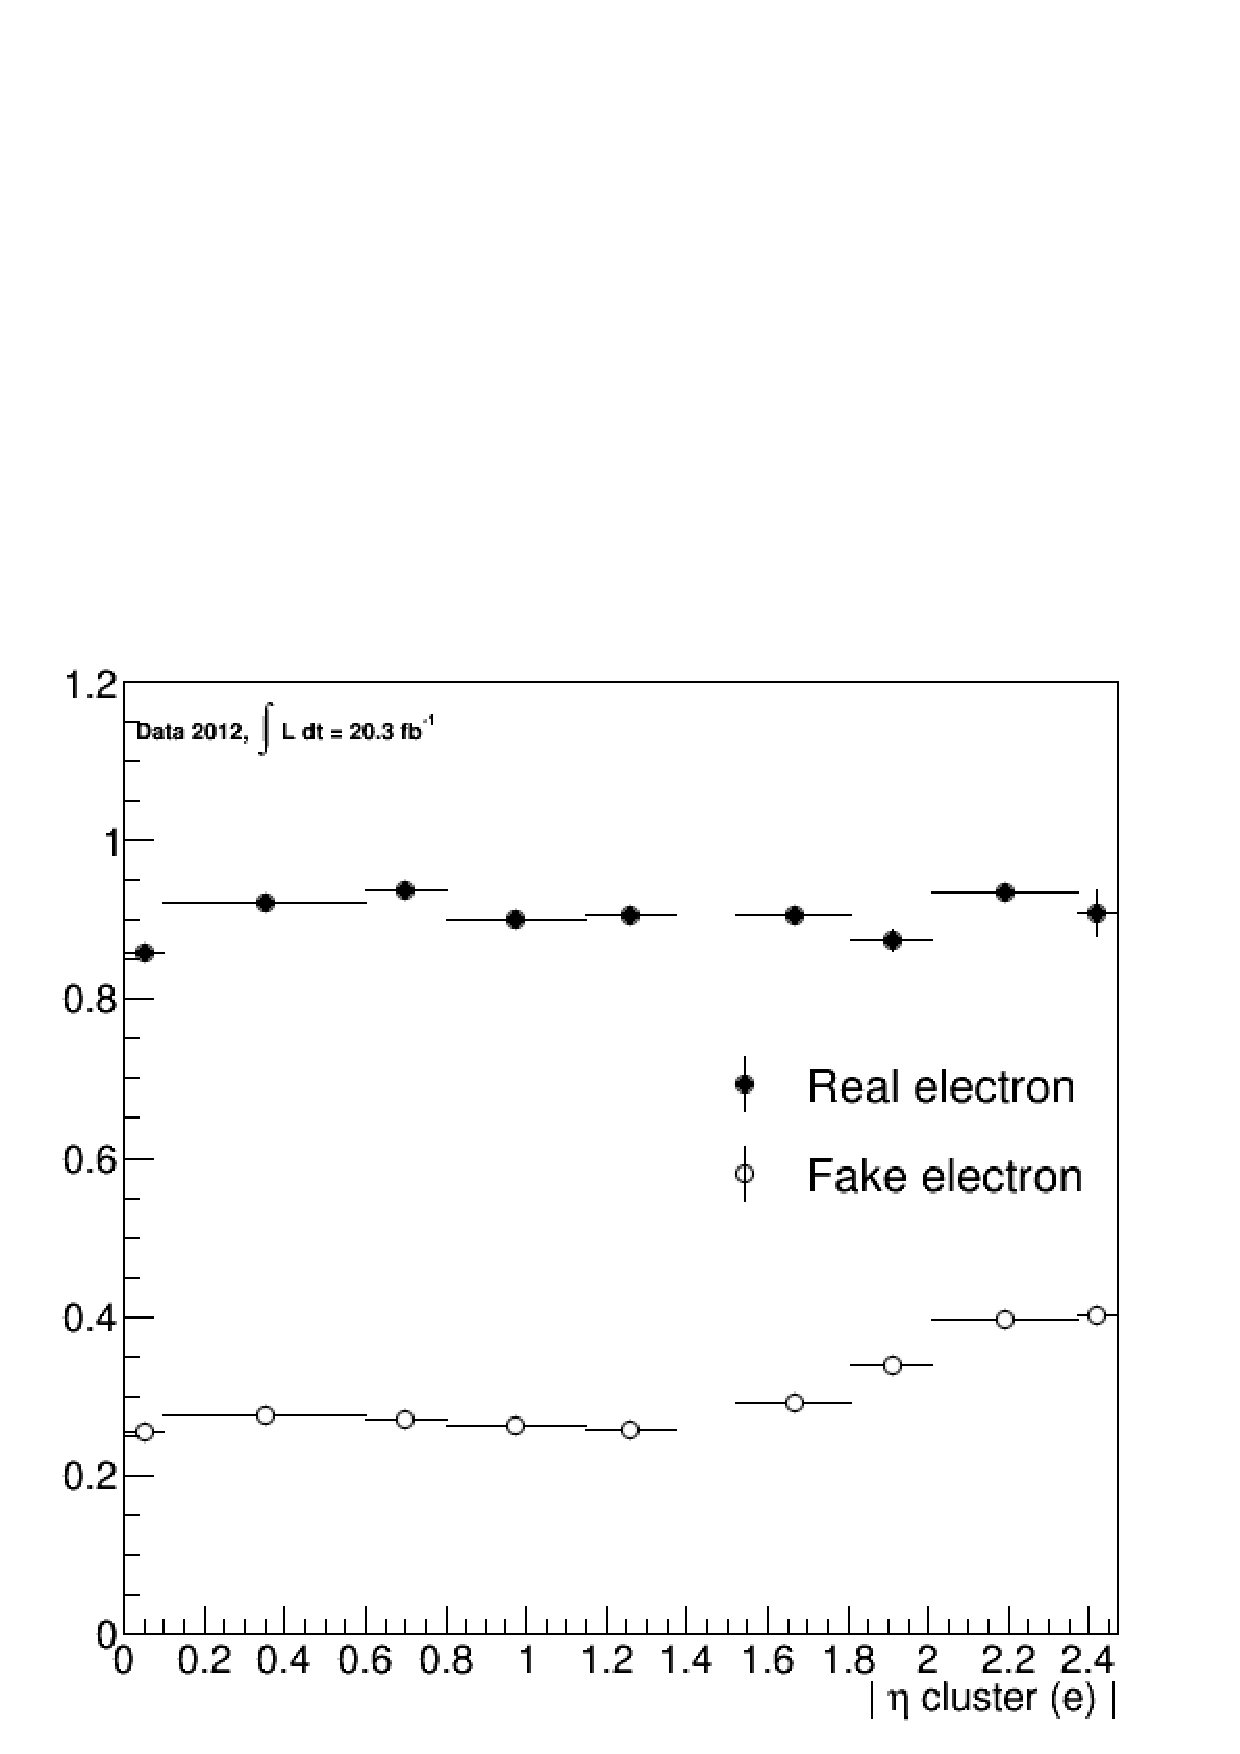
\includegraphics[width=0.4\textwidth]{Figures/Backgrounds/Eff_el_eta_CR2_realCR1_ge1tag_e24vhi.pdf}
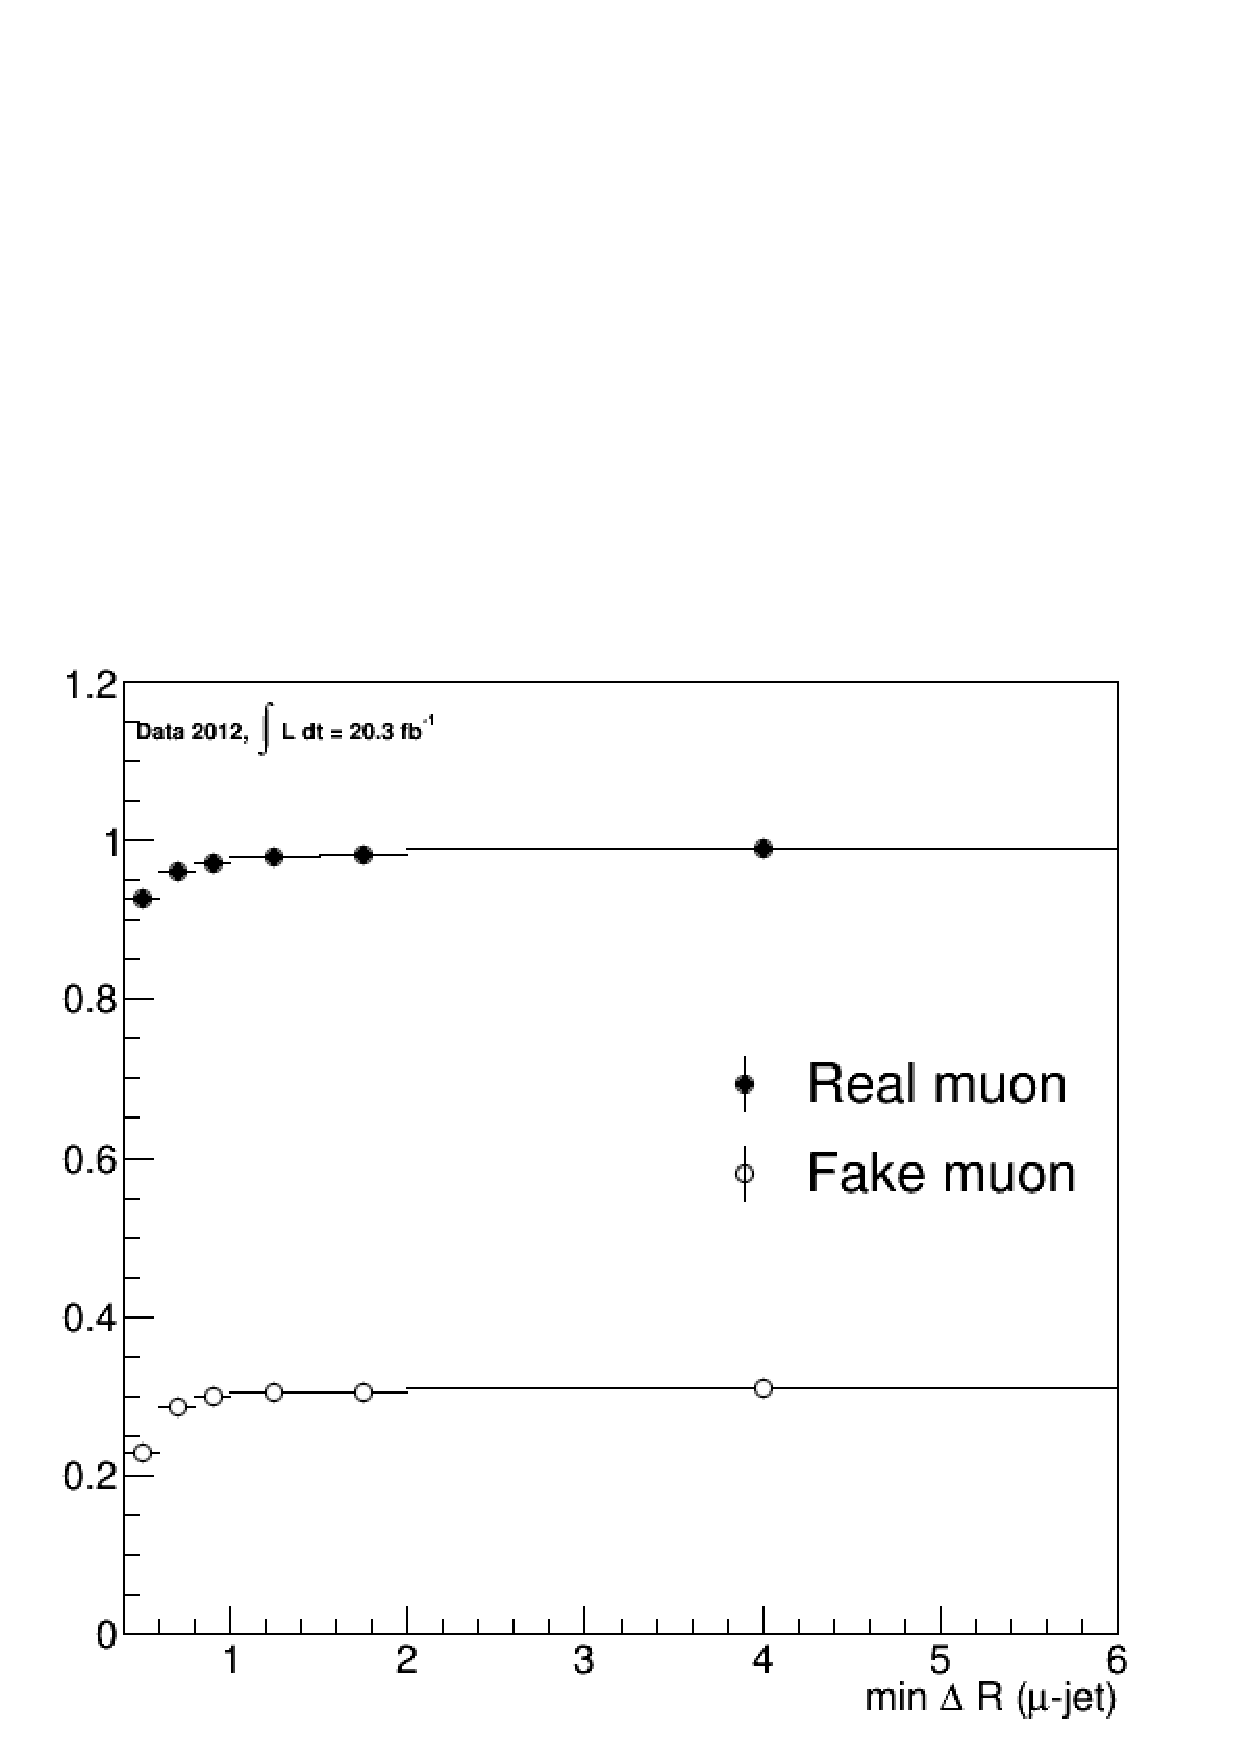
\includegraphics[width=0.4\textwidth]{Figures/Backgrounds/Eff_mu_dR_CR1_realCR1_mu24i.pdf}
\end{center}
\end{figure}

plot de gauche : $\geq 1$ b-jet, electrons matched to e24vhi \\
plot de droite : muons matched to mu24i
\end{frame}

\begin{frame}
\frametitle{Estimation des \english{fakes} : biais de trigger}

\begin{maliste}
\item Triggers utilisés :
\begin{itemize}
\item Electron stream: EF\_e24vhi\_medium1 or EF\_e60\_medium1
\item Muon stream: EF\_mu24i\_tight or EF\_mu36\_tight
\end{itemize} 
\item Triggers bas $p_T$ appliquent un critère d'isolation $\rightarrow$ $r$ et $f$ dépendent du trigger
\end{maliste}

\begin{tiny}
\begin{table}[htb]
  \begin{center}
%    \caption{Selection probabilities $r$ and $f$ applied to each lepton,  depending on the characteristics of the lepton and the event trigger.  High- and low-$p_T$ are defined here by the boundary between the $p_T$ thresholds of the triggers that require isolation and those that do not. For electrons, low-$p_T$ means the range 24 $< p_T <$ 61~GeV while for muons the range is 24 $< p_T <$ 37~GeV.}
    \begin{tabular}{cccc}
      \hline\hline
      Event trigger & $p_T$ rank among  &Lepton $p_T$ range  & Efficiency applied \\
                               & trigger-matched leptons &            &     \\ \hline
         $\ge 1$ lepton matches high-$p_T$ trigger & Any & high & high-$p_T$ \\
         $\ge 1$ lepton matches high-$p_T$ trigger & Any & low & low-$p_T$ unbiased \\
          No lepton matches high-$p_T$ trigger &   Leading  & Any & low-$p_T$ biased \\
          No lepton matches high-$p_T$ trigger &   Subleading & high & high-$p_T$ unbiased \\
          No lepton matches high-$p_T$ trigger &   Subleading & low & low-$p_T$ unbiased \\
                 \hline
        \end{tabular}
 \end{center}
\end{table}
\end{tiny}
\end{frame}

\begin{frame}
\frametitle{Estimation des \english{fakes} : canal di-leptonique}
\begin{footnotesize}
\[
\hspace*{-0.8cm}
\textcolor{red}{
\left( \begin{array}{c}
N^\mathrm{TT} \\
N^\mathrm{T\overline{T}} \\
N^\mathrm{\overline{T}T} \\
N^\mathrm{\overline{T}\overline{T}} \end{array} \right) 
}
= 
\underbrace{\left( \begin{array}{c c c c}
r_{1}r_{2} & r_{1}f_{2} & f_{1}r_{2} & f_{1}f_{2} \\
r_{1}\overline{r_{2}} & r_{1}\overline{f_{2}} & f_{1}\overline{r_{2}} & f_{1}\overline{f_{2}} \\
\overline{r_{1}}r_{2} & \overline{r_{1}}f_{2} & \overline{f_{1}}r_{2} & \overline{f_{1}}f_{2} \\
\overline{r_{1}}\overline{r_{2}} & \overline{r_{1}}\overline{f_{2}} & \overline{f_{1}}\overline{r_{2}} & \overline{f_{1}}\overline{f_{2}} \end{array} \right)}_{M}
\textcolor{blue}{
\left( \begin{array}{c}
N^\mathrm{LL}_\mathrm{RR} \\
N^\mathrm{LL}_\mathrm{RF} \\
N^\mathrm{LL}_\mathrm{FR} \\
N^\mathrm{LL}_\mathrm{FF} \end{array} \right)
}
\quad
\Longrightarrow 
\vspace*{0.2cm}
\textcolor{blue}{
\left( \begin{array}{c}
N^\mathrm{LL}_\mathrm{RR} \\
N^\mathrm{LL}_\mathrm{RF} \\
N^\mathrm{LL}_\mathrm{FR} \\
N^\mathrm{LL}_\mathrm{FF} \end{array} \right)
}
=
M^{-1}
\textcolor{red}{
\left( \begin{array}{c}
N^\mathrm{TT} \\
N^\mathrm{T\overline{T}} \\
N^\mathrm{\overline{T}T} \\
N^\mathrm{\overline{T}\overline{T}} \end{array} \right)
}
\]
\end{footnotesize}

\[\begin{split}
N^\mathrm{TT}_\mathrm{fake}   & = N^{TT}_\mathrm{RF} + N^\mathrm{TT}_\mathrm{FR} + N^\mathrm{TT}_\mathrm{FF} \\
                              & = r_1 f_2 N^\mathrm{LL}_\mathrm{RF} + f_1 r_2 N^\mathrm{LL}_\mathrm{FR} + f_1 f_2 N^\mathrm{LL}_\mathrm{FF}
\end{split}\]

\end{frame}

\begin{frame}
\frametitle{Estimation des \english{fakes} : canal tri-leptonique}
\begin{scriptsize}
\[
\hspace*{-0.8cm}
\textcolor{red}{
\left( \begin{array}{c}
N^\mathrm{TTT} \\
N^\mathrm{TT\overline{T}} \\
N^\mathrm{T\overline{T}T} \\
N^\mathrm{T\overline{T}\overline{T}} \\
N^\mathrm{\overline{T}TT} \\
N^\mathrm{\overline{T}T\overline{T}} \\
N^\mathrm{\overline{T}\overline{T}T} \\
N^\mathrm{\overline{T}\overline{T}\overline{T}} \\
\end{array} \right)}
=
\left( \begin{array}{cccccccc}
r_1r_2r_3 & r_1r_2f_3 & r_1f_2r_3 & r_1f_2f_3 &  f_1r_2r_3 & f_1r_2f_3 & f_1f_2r_3 & f_1f_2f_3 \\

r_1r_2\overline{r_3} & r_1r_2\overline{f_3} & r_1f_2\overline{r_3} & r_1f_2\overline{f_3} &  f_1r_2\overline{r_3} & f_1r_2\overline{f_3} & f_1f_2\overline{r_3} & f_1f_2\overline{f_3} \\

r_1\overline{r_2}r_3 & r_1\overline{r_2}f_3 & r_1\overline{f_2}r_3 & r_1\overline{f_2}f_3 &  f_1\overline{r_2}r_3 & f_1\overline{r_2}f_3 & f_1\overline{f_2}r_3 & f_1\overline{f_2}f_3 \\

r_1\overline{r_2}\overline{r_3} & r_1\overline{r_2}\overline{f_3} & r_1\overline{f_2}\overline{r_3} & r_1\overline{f_2}\overline{f_3} &  f_1\overline{r_2}\overline{r_3} & f_1\overline{r_2}\overline{f_3} & f_1\overline{f_2}\overline{r_3} & f_1\overline{f_2}\overline{f_3} \\

\overline{r_1}r_2r_3 & \overline{r_1}r_2f_3 & \overline{r_1}f_2r_3 &\overline{r_1}f_2f_3 &  \overline{f_1}r_2r_3 & \overline{f_1}r_2f_3 & \overline{f_1}f_2r_3 & \overline{f_1}f_2f_3 \\

\overline{r_1}r_2\overline{r_3} & \overline{r_1}r_2\overline{f_3} & \overline{r_1}f_2\overline{r_3} & \overline{r_1}f_2\overline{f_3} &  \overline{f_1}r_2\overline{r_3} & \overline{f_1}r_2\overline{f_3} & \overline{f_1}f_2\overline{r_3} & \overline{f_1}f_2\overline{f_3} \\

\overline{r_1}\overline{r_2}r_3 & \overline{r_1}\overline{r_2}f_3 & \overline{r_1}\overline{f_2}r_3 & \overline{r_1}\overline{f_2}f_3 &  \overline{f_1}\overline{r_2}r_3 & \overline{f_1}\overline{r_2}f_3 & \overline{f_1}\overline{f_2}r_3 & \overline{f_1}\overline{f_2}f_3 \\

\overline{r_1}\overline{r_2}\overline{r_3} & \overline{r_1}\overline{r_2}\overline{f_3} & \overline{r_1}\overline{f_2}\overline{r_3} & \overline{r_1}\overline{f_2}\overline{f_3} & \overline{f_1}\overline{r_2}\overline{r_3} & \overline{f_1}\overline{r_2}\overline{f_3} & \overline{f_1}\overline{f_2}\overline{r_3} & \overline{f_1}\overline{f_2}\overline{f_3}

\end{array} \right)
\textcolor{blue}{
\left( \begin{array}{c}
N^\mathrm{LLL}_\mathrm{RRR} \\
N^\mathrm{LLL}_\mathrm{RRF} \\
N^\mathrm{LLL}_\mathrm{RFR} \\
N^\mathrm{LLL}_\mathrm{RFF} \\
N^\mathrm{LLL}_\mathrm{FRR} \\
N^\mathrm{LLL}_\mathrm{FRF} \\
N^\mathrm{LLL}_\mathrm{FFR}\\
N^\mathrm{LLL}_\mathrm{FFF}
\end{array} \right)}
\]
\end{scriptsize}

\[
\begin{split}
N_\mathrm{fake}^\mathrm{TTT} &= N^\mathrm{TTT}_\mathrm{RRF} + N^\mathrm{TTT}_\mathrm{RFR}+N^\mathrm{TTT}_\mathrm{RFF}+N^\mathrm{TTT}_\mathrm{FRR} + N^\mathrm{TTT}_\mathrm{FRF} + N^\mathrm{TTT}_\mathrm{FFR} +N^\mathrm{TTT}_\mathrm{FFF} \\   
                             &= r_1r_2f_3N^\mathrm{LLL}_\mathrm{RRF} + r_1f_2r_3N^\mathrm{LLL}_\mathrm{RFR} +r_1f_2f_3N^\mathrm{LLL}_\mathrm{RFF}+f_1r_2r_3N^\mathrm{LLL}_\mathrm{FRR} \\
                             &\quad f_1r_2f_3N^\mathrm{LLL}_\mathrm{FRF} + f_1f_2r_3N^\mathrm{LLL}_\mathrm{FFR} +f_1f_2f_3N^\mathrm{LLL}_\mathrm{FFF}
\end{split}
\]

\end{frame}



\begin{frame}
\frametitle{Estimation des \english{fakes} : incertitude systématiques}

\begin{maliste}
\item Sources d'incertitudes sur $r$ et $f$ considérées :
\begin{itemize}
\item Définition des régions pour détermination de $r$ et $f$ : $\ETmiss<20$~GeV pour $f$ des électrons, $m_T(W)<20$~GeV et $m_T(W)+\ETmiss<60$~GeV pour $f$ des muons, $\ETmiss>175$~GeV pour $r$ des électrons et $m_T(W)>110$~GeV pour $r$ des muons.
\item MC utilisé pour mesure de $f$ (normalisation variée de $\pm$10\%)
\item Statistique pour $r$ et $f$ : échantillons divisés en 4 pour 4 détermination indépendante de $r$ et $f$. \english{Fakes} yield estimée 4 fois et erreur estimée en calculant déviation standard de ces 4 estimations (divisée par 2).
\end{itemize}
\item Ces incertitudes sur $r$ et $f$ ont été propagées à l'estimation du nombre de \english{fakes}.
\item Incertitude finale conservative : 70\%.
\end{maliste}
\end{frame}

\begin{frame}
\frametitle{Estimation des \english{mis-id} : détermination des taux}

\begin{maliste}
\item Négligeable pour les muons : $\varepsilon_\mu=\text{qq}~10^{-5}$ ($\varepsilon_\mu\simeq 100 \varepsilon_e$)
\item Sources pour électrons : 
\begin{itemize}
\item erreur due au grand rayon de courbure pour électron de haute énergie 
\item électrons tridents
\end{itemize}
\item \'Echantillon pour déterminer rates : $Z(\rightarrow ee)$+jets
\item Paramétrisation : $\eta$, $p_T$
\item Détermination par maximum de vraisemblance : 
\begin{itemize}
\item $N_{\text{ss}}\sim Poisson\left(N\left(\varepsilon_1+\varepsilon_2\right)\right)$ ($N$ = nb evts avec 2 leptons de charges vraies opposées)
\item $ln[{\cal L}(\varepsilon | N_{ss},N)] = \sum_{i,j} ln[(\varepsilon_i + \varepsilon_j)N^{i,j}]N_{\text{ss}}^{i,j} - (\varepsilon_{i} + \varepsilon_{j})N^{i,j}$
\end{itemize}
\end{maliste}
\end{frame}


\begin{frame}
\frametitle{Estimation des \english{mis-id} : détermination des taux}
\begin{small}
\[
\hspace*{-0.5cm}
\varepsilon\left(|\eta|,p_T>100~\text{GeV}\right)=\varepsilon\left(|\eta|,p_T\in\left[80,100\right]~\text{GeV}\right)\times\underbrace{\frac{\varepsilon_{t\bar{t}}\left(|\eta|,p_T>100~\text{GeV}\right)}{\varepsilon_{t\bar{t}}\left(|\eta|,p_T\in\left[80,100\right]~\text{GeV}\right)}}_{\alpha_{t\bar{t}}}\]
\end{small}

\begin{figure}[!htb]
\begin{center}
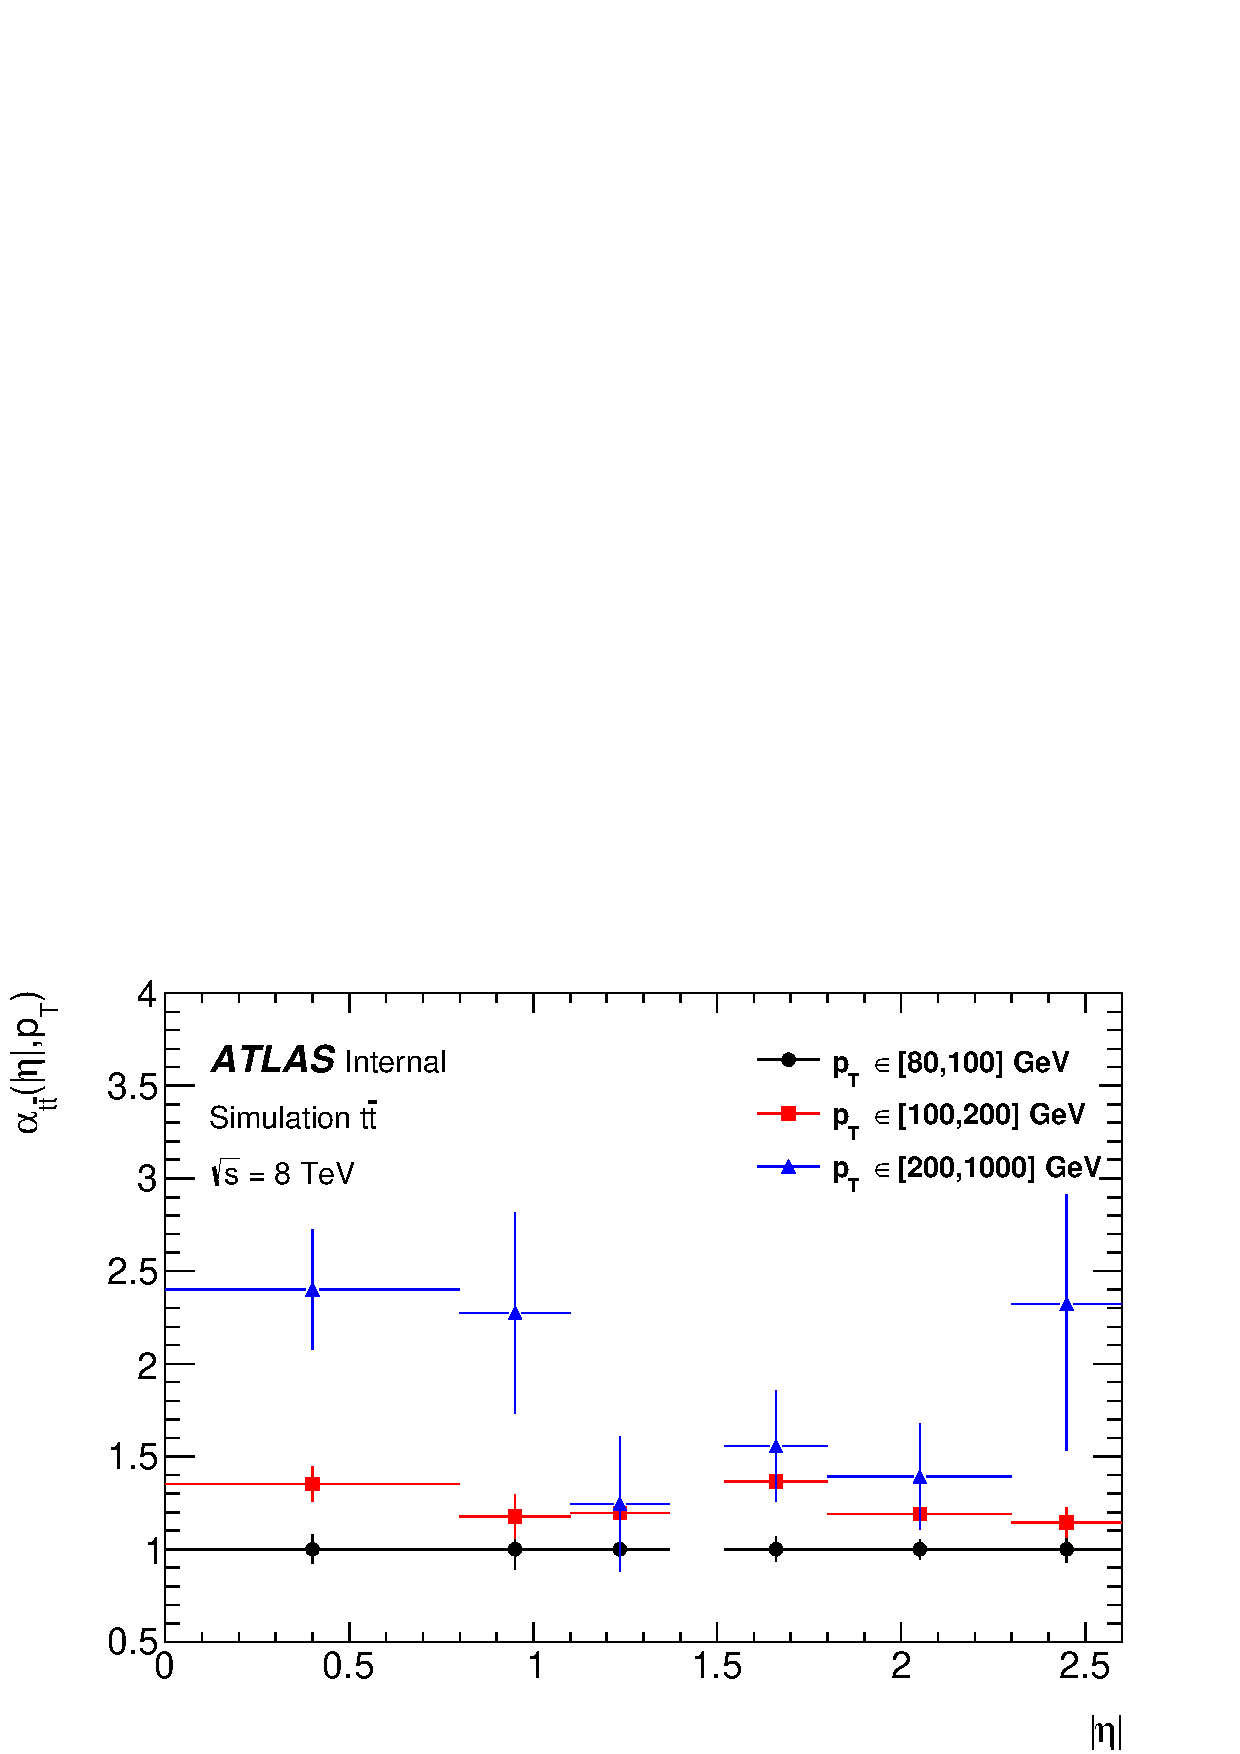
\includegraphics[width=0.5\textwidth]{Figures/QMisId/alpha.pdf}
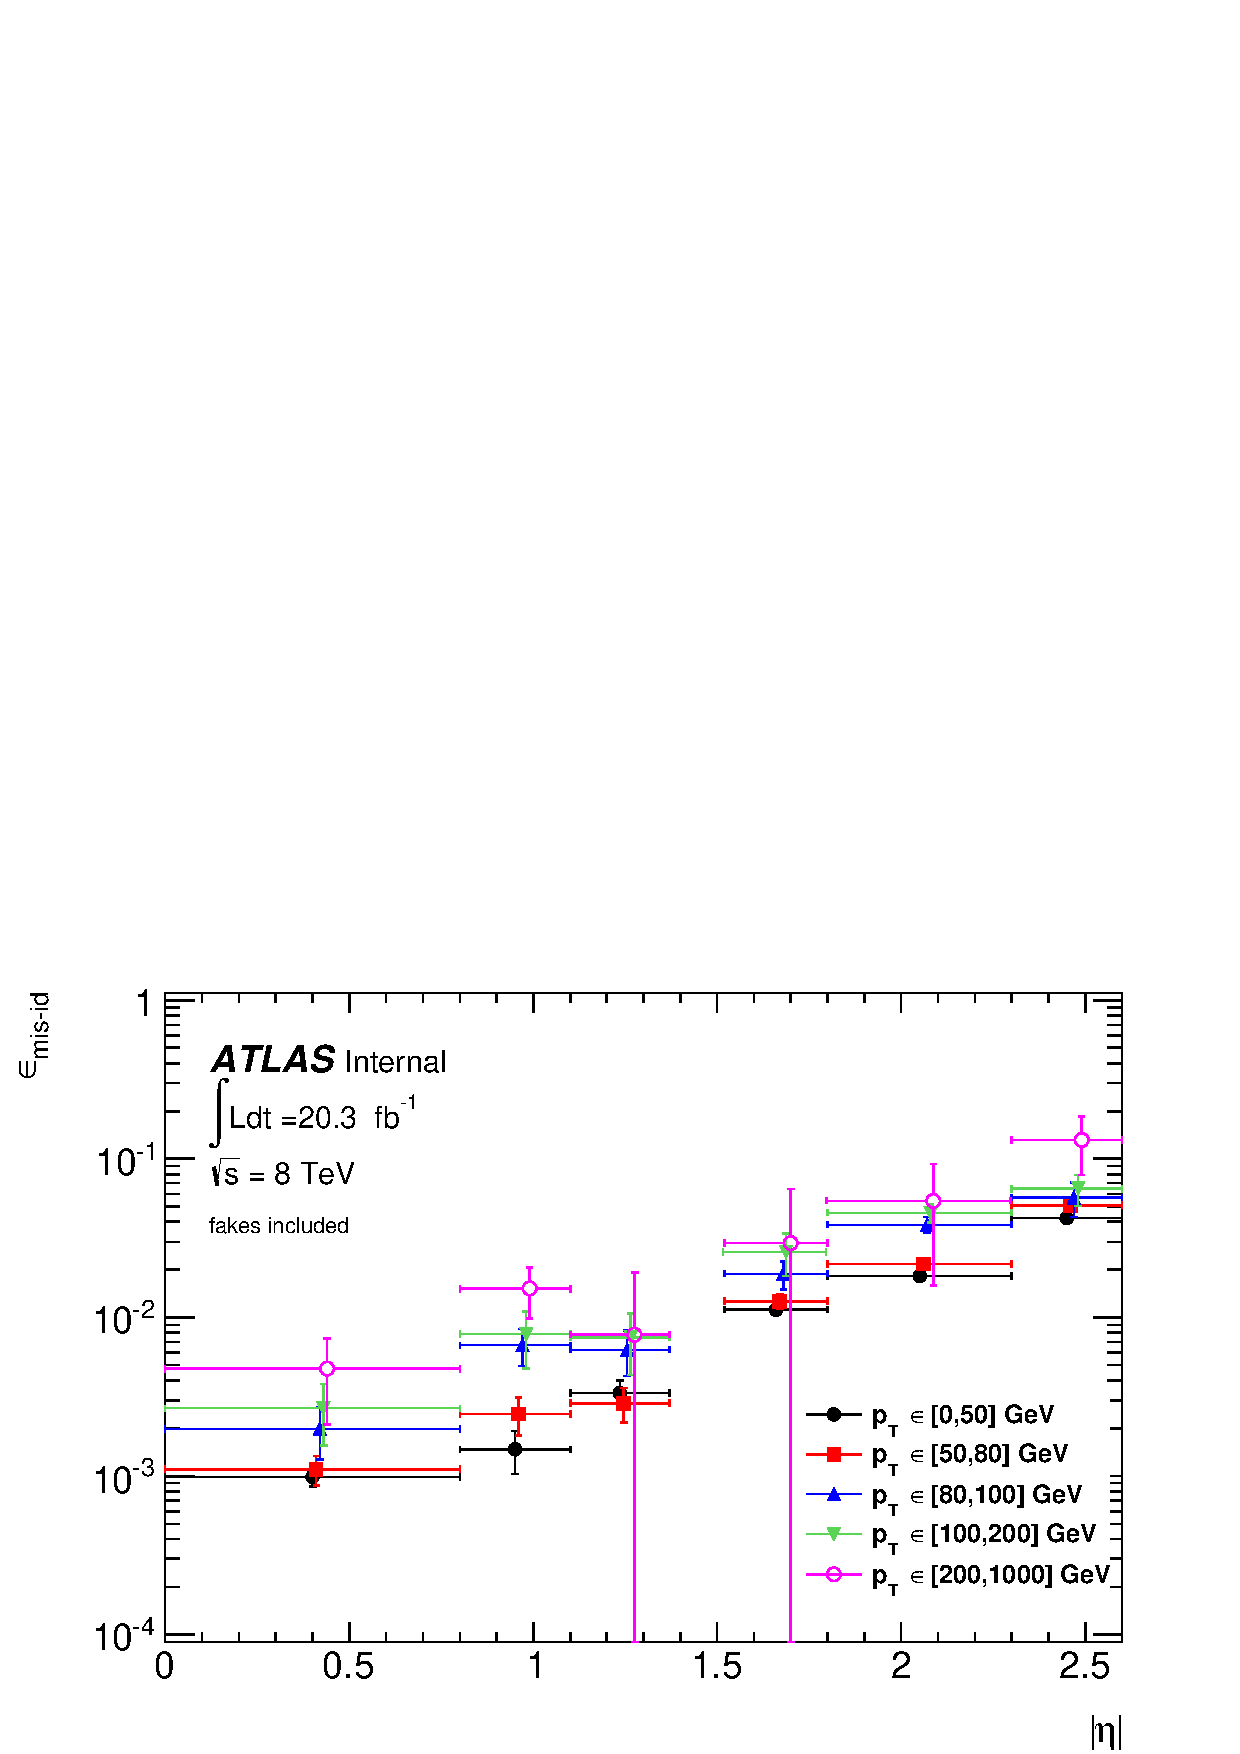
\includegraphics[width=0.5\textwidth]{Figures/QMisId/Rates2DwithFakes.pdf}
\end{center}
\end{figure}

\end{frame}

\begin{frame}
\frametitle{Estimation des \english{mis-id} : détermination des yields}
\begin{maliste}
\item Estimation à partir d'événements de charges opposées :
\begin{itemize}
\item $N_{\text{ss}} = \left[\varepsilon_i(1-\varepsilon_j) + \varepsilon_j(1-\varepsilon_i)\right]N \simeq \left(\varepsilon_i+\varepsilon_j\right)N$
\item $N_{\text{os}} = \left[\left(1-\varepsilon_i\right)\left(1-\varepsilon_j\right)+\varepsilon_i\varepsilon_j\right]N$
\end{itemize}
Donc
\begin{itemize}
\item $N_{\text{ss}} = \frac{\varepsilon_i(1-\varepsilon_j) + \varepsilon_j(1-\varepsilon_i)}{\left(1-\varepsilon_i\right)\left(1-\varepsilon_j\right)+\varepsilon_i\varepsilon_j}N_{\text{os}}$
\end{itemize}
\end{maliste}

\begin{figure}[p]
  \begin{center}
    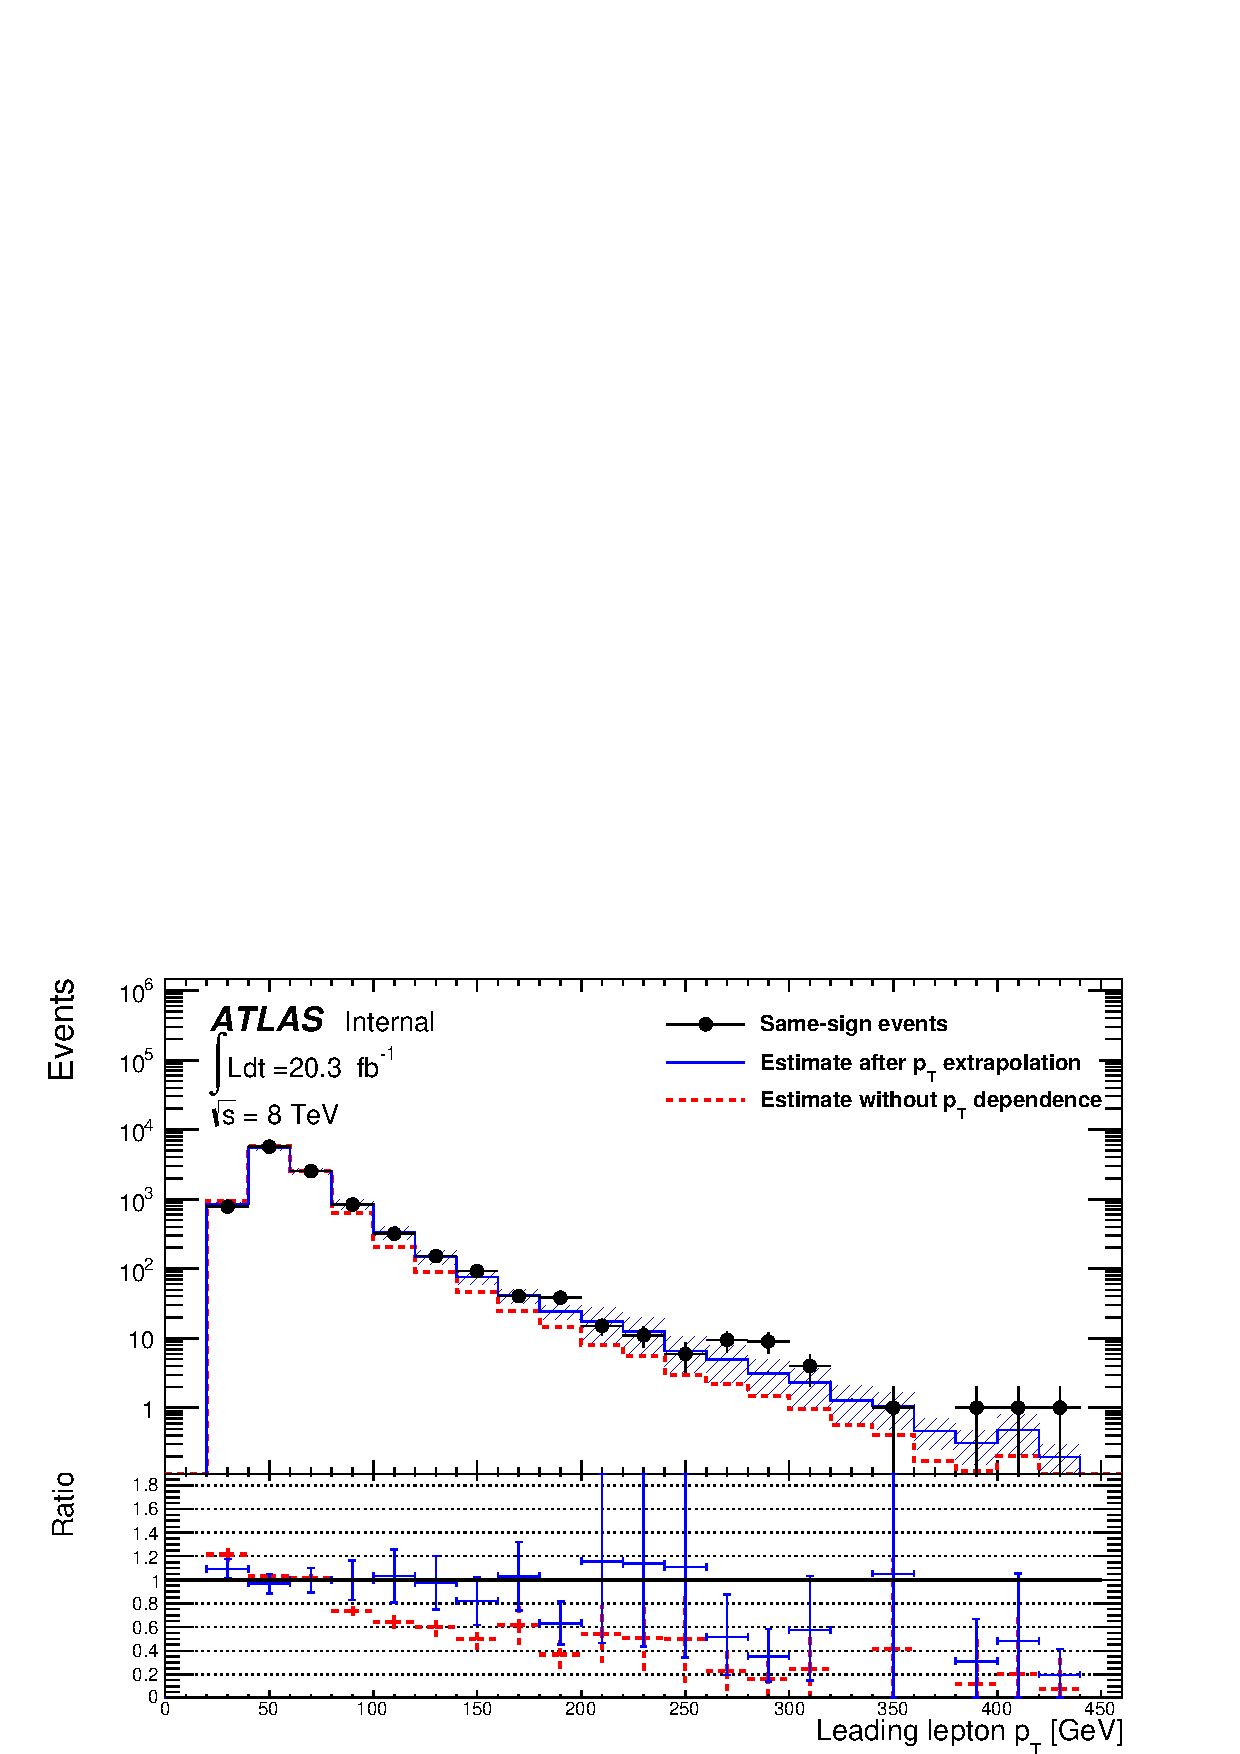
\includegraphics[width=0.65\textwidth]{Figures/QMisId/ClosureDataPtR.pdf}
  \end{center}
%  \caption{Distribution in data of the leading electron \pt{} for $Z$ events. The $e^{\pm}e^{\pm}$ events are displayed as black points. The charge mis-id estimate using reweighted $e^+e^-$ events is shown with the red-dashed line when no \pt-dependence is applied (i.e. the charge mis-id rates are determined without any \pt{} dependence in the likelihood and no \pt{} correction factor is applied) and with the blue line when the \pt-dependence is applied.}\label{fig:QMid:ratePt}
\end{figure}
\end{frame}

\begin{frame}
\frametitle{Estimation des \english{mis-id} : incertitudes systématiques}

\begin{maliste}
\item 6 sources d'incertitudes sur rates considérées :
\begin{itemize}
\item incertitude stat. issue de l'estimation par maximum de vraisemblance
\item incertitude stat. sur facteur correctif $\alpha_{t\bar{t}}$ à haut $p_T$  
\item différence des rates maximum vraisemblance et des rates truth sur événements $Z\rightarrow e^+e^-$ simulés
\item différence des rates entre électrons et positons (si ces rates diffèrent de plus de $1\sigma$
\item définition du pic du $Z$
\item échantillon $t\bar{t}$ (MC@NLO+Herwig au lieu de POWHEG+Pythia) pour détermination du facteur correctif $\alpha_{t\bar{t}}$ à haut $p_T$
\end{itemize}
\item Incertitude totale sur rates ($\sigma$) = somme quadratique de ces 6 contributions
\item Incertitude sur yield calculée en faisant varier rates de $\pm 1\sigma$
\end{maliste}

\end{frame}


\begin{frame}
\frametitle{\english{Fakes/mis-id} overlap removal}

\begin{figure}[p]
  \begin{center}
%\subfigure[Ratio between the charge mis-id rates after and before removing the fakes component.\label{fig:QMid:overlap}]{
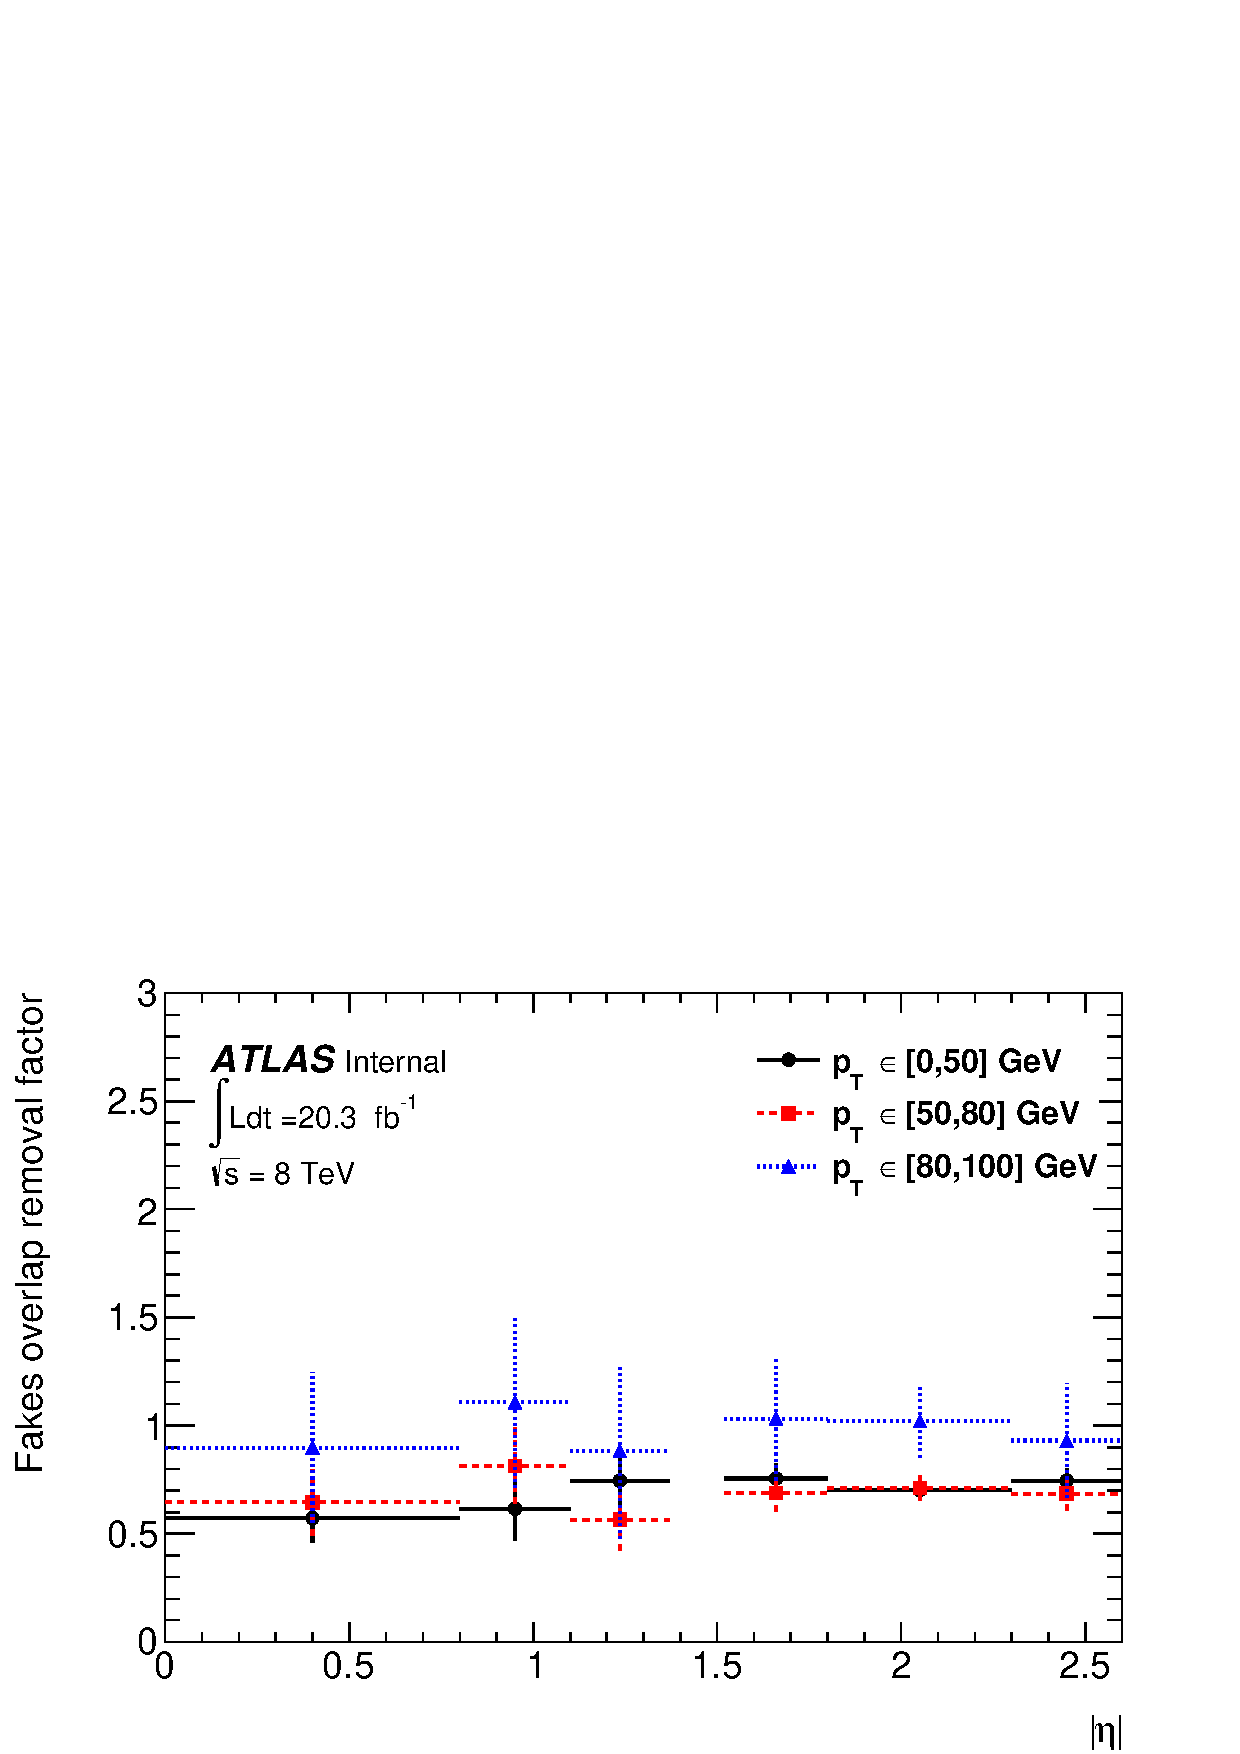
\includegraphics[width=0.5\textwidth]{Figures/QMisId/Overlap.pdf}
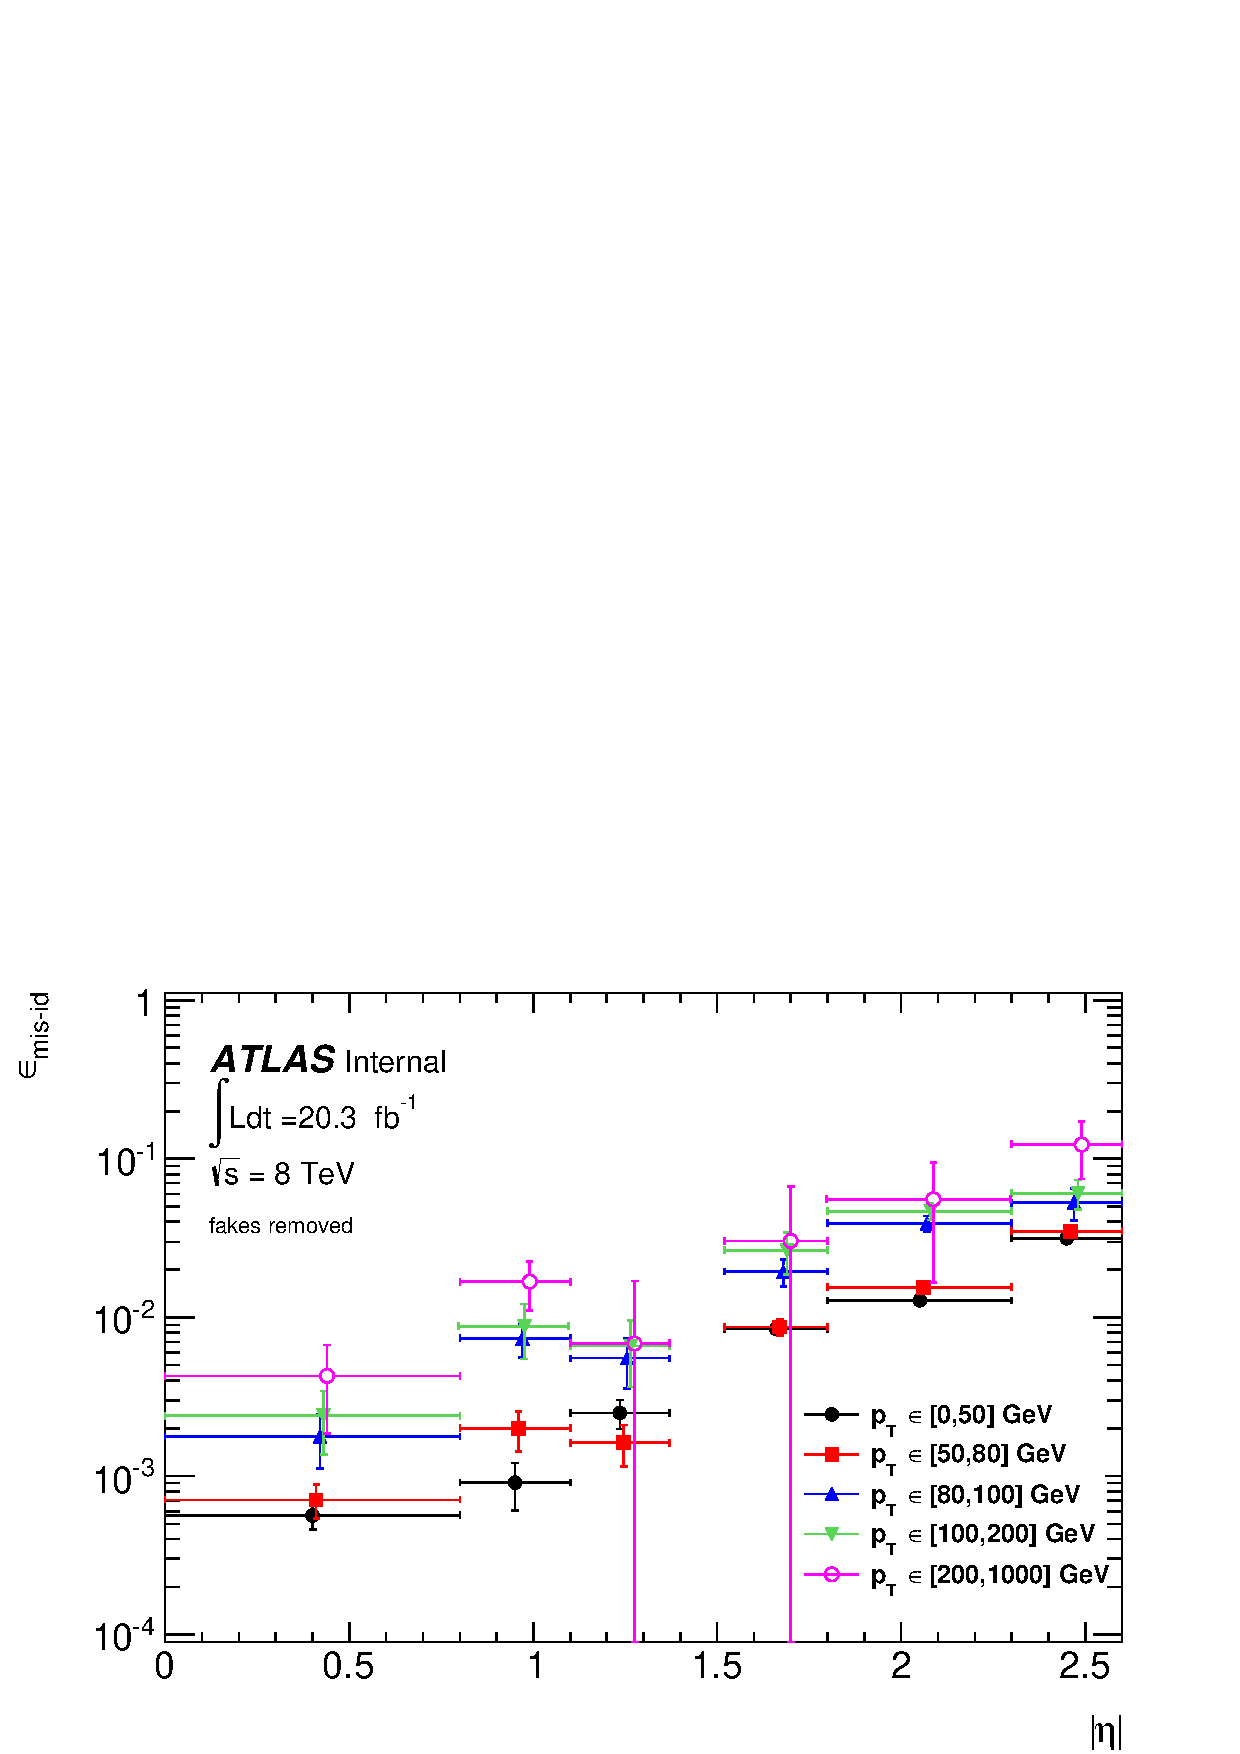
\includegraphics[width=0.5\textwidth]{Figures/QMisId/Rates2DwithoutFakes.pdf}
  \end{center}
%  \caption{Removal of fakes in the charge mis-id rates.}
\end{figure}
\end{frame}

\begin{frame}
\frametitle{\english{Fakes/mis-id} overlap removal : incertitude systématique}

\begin{maliste}
\item Rates \english{mis-id} recalculés en faisant varier les $r$ et $f$ utilisés pour l'estimation et la soustraction des \english{fakes}
\item Sources d'incertitudes sur $r$ et $f$ sont celles considérées pour l'estimation de l'incertitude sur les \english{fakes}
\end{maliste}
\end{frame}

\begin{frame}
\frametitle{Vérification estimation fonds}
\begin{maliste}
\item Détailler toutes les verifs faites pour s'assurer que l'exces n'est pas lie à une mauvaise modelisation
\end{maliste}
\end{frame}

\begin{frame}
\frametitle{Yields}
\begin{table}[!htb]
  \begin{center}
  \scalebox{0.6}{    \begin{tabular}{|l | c | c | c | c |c | }
      \cline{2-6}%\cline{2-6}
       \multicolumn{1}{c|}{ } & {\bf SR4t0} & {\bf SR4t1} & {\bf SR4t2} & {\bf SR4t3} & {\bf SR4t4} \\ \cline{2-6}
       \multicolumn{6}{c}{\bf Signaux} \\
      \hline
 %     $m_{KK}=600$~GeV & $7,7 \pm 1,3 $ & $5,9 \pm 1,1 $ & $81 \pm 4 $ & $321 \pm 9 $ & $588 \pm 11 $\\
 %     $m_{KK}=800$~GeV & $0,08 \pm 0,04 $ & $0,12 \pm 0,05 $ & $6,9 \pm 0,4 $ & $38,7 \pm 0,9 $ & $60,9 \pm 1,0 $\\
      $m_{KK}=1000$~GeV & $ ( 9 \pm 5) \cdot 10^{-3}  $ & $ ( 5 \pm 5) \cdot 10^{-4}  $ & $0,77 \pm 0,05 $ & $5,02 \pm 0,12 $ & $6,72 \pm 0,13 $\\
%      $m_{KK}=1200$~GeV & $< 1,9 \cdot 10^{-4}$ & $< 1,9 \cdot 10^{-4}$ & $ ( 74 \pm 5) \cdot 10^{-3}  $ & $0,648 \pm 0,014 $ & $0,689 \pm 0.013 $\\
\hline
 Mod\`ele standard   & $ ( 42,8 \pm 2,1) \cdot 10^{-3}  $ & $ ( 38,8 \pm 2.0) \cdot 10^{-3}  $ & $ ( 25,8 \pm 1.7) \cdot 10^{-3}  $ & $ ( 58,3 \pm 2.7) \cdot 10^{-3}  $ & $ ( 105,7 \pm 3.4) \cdot 10^{-3}  $\\
      \hline
      Interaction contact & $1,60 \pm 0,10 $                  & $1,26 \pm 0,09 $                  & $1,96 \pm 0,12 $                   & $5,26 \pm 0,20 $                    & $8,88 \pm 0,24 $  \\
      \hline
      \multicolumn{6}{c}{\bf Bruits de fond} \\
      \hline

       $t\bar{t}W/Z$            & $12.6 \pm 0.3 \pm 5.4$       & $1.24 \pm 0.09\pm 0.53$& $1.87 \pm 0.09\pm 0.80$ & $2.46 \pm 0.11\pm 1.06$ & $0.57\pm 0.05 \pm 0.25$ \\
      $t\bar{t}H$                & $1.8 \pm 0.1 \pm 0.2$           & $ 0.26 \pm 0.03 \pm 0.05$&  $0.31 \pm 0.04\pm 0.05$ & $0.44\pm 0.04\pm 0.06$ & $0.08\pm 0.02\pm 0.02$\\
       Dibosons                    & $0.95 \pm 0.19\pm 0.25$       & $0.07 \pm 0.12 \pm 0.05$ & $0.33\pm 0.14\pm 0.10$ & $0.04\pm 0.12\pm 0.03$ & $0.00\pm 0.12\pm 0.00$ \\
       Fake/Non-prompt   & $8.61 \pm 2.34 \pm 5.02$ & $1.17 \pm 0.82 \pm 0.68$&  $1.03\pm 0.97 \pm 0.60$ & $0.00\pm 1.02 \pm 0.28$ & $0.04\pm 0.83 \pm 0.24$\\    
       Q mis-Id                    & $15.1 \pm 0.6 \pm 3.5$           & $0.74 \pm 0.11 \pm 0.18$&  $1.17\pm 0.16 \pm 0.38$ & $1.09\pm 0.14 \pm 0.34$ & $0.30\pm 0.09 \pm 0.10$\\  
      Autres                        & $0.75 \pm 0.04 \pm 0.10$      & $0.10 \pm 0.08 \pm 0.03$ &  $0.16\pm 0.08\pm 0.02$ & $0.23\pm 0.08\pm 0.05$ & $0.14\pm 0.08\pm 0.08$\\        
%\hdashline
\hline
       Total               & $40.0 \pm 2.4 \pm 7.3 $ & $3.6 \pm 0.9 \pm 0.8$ & $4.9 \pm 1.0 \pm 1.0 $ & $4.3 \pm 1.1 \pm 1.1 $ & $1.1 \pm 0.9 \pm 0.4 $\\

      \hline
       \multicolumn{6}{c}{\bf Observ\'e} \\ \cline{2-6}
       \multicolumn{1}{c|}{}                         & 54 & 6 & 6 & 12 & 6 \\ \cline{2-6}
    \end{tabular}}
%    \caption{Nombre d'\'ev\'enements attendu pour les signaux recherchés et les bruits de fond et nombre d'événements observés dans les diff\'erentes r\'egions de signal. Les incertitudes sur les nombres d'\'ev\'enements pour les signaux sont les incertitudes statistiques. Pour les bruits de fond, les premi\`eres et deuxi\`emes incertitudes sont respectivement les incertitudes statistiques et syst\'ematiques (ces derni\`eres sont donn\'ees par l'\'ecart-type de la distribution marginale du nombre d'\'ev\'enements). Pour la production par interaction de contact, les nombres donn\'es ont \'et\'e obtenus avec $C/\Lambda^2=-4\pi$~TeV$^{-2}$.\label{tab:allYields}}
  \end{center}
\end{table}

Mettre plutot table en backup et figure a la place ?
\end{frame}

\begin{frame}
\frametitle{4 tops analysis in lepton+jets channel ATLAS (arXiv:1505.04306)}

\begin{columns}
\begin{column}{0.6\textwidth}
\begin{maliste}
\item Selection :
\begin{itemize}
\item Same triggers as in our analysis
\item exactly $1$ lepton ($e$ or $\mu$)
\item $\geq 5$ jets
\item $\geq 2$ b-tagged jets 
\item $\met\geq$ 20 GeV
\item $\met + m_T^W \geq 60$ GeV
\item Categories : $5$ and $\geq~6$ jet, $2,3$ and $\geq 4$ b-tagged jets
\end{itemize}
\vspace*{0.2cm}
\item Backgrounds :
\begin{itemize}
\item $t\bar{t}+$jets
\item $W$+jets
\item multijets
\item single-top, $Z$+jets, $VV$, $t\bar{t}V$, $t\bar{t}H$
\end{itemize}
\end{maliste}
\end{column}
\begin{column}{0.5\textwidth}
\begin{maliste}
\item Statistical analysis : pure frequentist, $H_T$ fit ($H_T$ includes \met)
\vspace*{0.2cm}
\item Results : 
\begin{itemize}
\item SM $tt\bar{t}\bar{t}$ : $23~$fb ($32$~fb) observed (expected)
\item CI $tt\bar{t}\bar{t}$ : $12~$fb ($16$~fb) observed (expected)
\item 2UED/RPP : $m_{KK} > 1.12~$TeV ($1.10$~TeV) observed (expected)
\end{itemize}
\end{maliste}
\end{column}
\end{columns}
\end{frame}

\begin{frame}
\frametitle{4 tops analysis in lepton+jets channel CMS (arXiv:1409.7339)}
\begin{columns}
\begin{column}{0.5\textwidth}
\begin{maliste}
\item Data: $19.6~$fb$^{-1}$ at $8$~TeV
\item Channel: lepton ($e$ or $\mu$) +jets
\item Signal simulation: MadGraph5 v1.3.30
\item Backgrounds
\begin{itemize}
\item $t\bar{t}+0,1,2,3$~partons ($t\bar{t}$ decays considered:$0,1,2$ leptons)
\item $t\bar{t}+V$
\item $W/Z$+partons
\item single-top
\item $t\bar{t}H$
\item $VV$
\end{itemize}
\item Objets:
\begin{itemize}
\item jets: \antikt~$R=0.5$
\end{itemize}
\end{maliste}
\end{column}
\begin{column}{0.5\textwidth}
\begin{maliste}
\item Selection :
\begin{itemize}
\item $1$ electron or muon ($p_T>30~$GeV)
\item $\geq 6$ jets ($p_T>30~$GeV)
\item $\geq 2$ b-tagged jets
\item $H_T=\sum\limits_{jets}p_T >400$~GeV
\item $\met > 30$~GeV
\end{itemize}
\item Analysis: kinematic reconstruction + multivariate techniques
\item Statistical analysis: pure frequentist, BDT$_\text{event}$ fit
\item Results: 
\begin{itemize}
\item $\sigma<32~$fb ($32\pm 17$~fb) observed (expected)
\end{itemize}
\end{maliste}
\end{column}
\end{columns}

\end{frame}


\begin{frame}
\frametitle{Same-sign dilepton excesses in ATLAS and CMS}

\begin{maliste}
\item Following data extracted from arXiv:1507.01601: {\it Same-Sign Dilepton Excesses and Light Top Squarks}, P. Huang, A. Ismail, I. Low, C. Wagner
\end{maliste}

\begin{table}[!htb]
  \begin{center}
   \scalebox{0.6}{    
  \begin{tabular}{|c|c|c|c|c|c|c|c|}
  \cline{2-8}
\multicolumn{1}{c|}{} & $N_{b-\text{jets}}$  & $N_\text{jets}$           & $\met$            & $H_T$          & $m_\text{eff}$ & $m_T^W$        & Comments         \\ \hline
CMS SUSY              & $\geq 2$             & $\geq 4$                  & $\in[50,120]$~GeV & $\geq 400$~GeV & $-$            & $-$            & No \pval{} given \\ 
arXiv:1311.6736       & & & & & & & \\ \hline 
ATLAS SUSY            & $1,2$                & $\geq 3$                  & $\geq 150$~GeV    & $-$            & $\geq 700~$GeV & $\geq 100~$GeV & $\pval=0.07$     \\ 
arXiv:1404.2500       & & & & & & & \\ \hline 
CMS $t\bar{t}H$       & $\geq 1$             & $\geq 4$                  & $-$               & $-$            & $-$            & $-$            & $\mu=5.3\pm^{+2.1}_{-1.8}$ \\ 
arXiv:1408.1682       & & & & & & & \\ \hline 
ATLAS Exotic $4t3$    & $=2$                 & $\geq 2$                  & $\geq 100$~GeV    & $\geq 700$~GeV & $-$            & $-$            & $\pval=0.029$ \\ 
arXiv:1504.04605      & & & & & & & \\ \hline 
ATLAS $t\bar{t}H$     & $\geq 1$             & $\geq 4$                  & $-$               & $-$             & $-$            & $-$           & $\mu=2.8\pm^{+2.1}_{-1.9}$ \\ 
arXiv:1506.05988      & & & & & & & \\ \hline 
\end{tabular}
}
\end{center}
\end{table}

\end{frame}


